% Options for packages loaded elsewhere
\PassOptionsToPackage{unicode}{hyperref}
\PassOptionsToPackage{hyphens}{url}
\PassOptionsToPackage{dvipsnames,svgnames,x11names}{xcolor}
%
\documentclass[
  12pt,
  a4paperpaper,
  a4paper]{scrreprt}

\usepackage{amsmath,amssymb}
\usepackage{setspace}
\usepackage{iftex}
\ifPDFTeX
  \usepackage[T1]{fontenc}
  \usepackage[utf8]{inputenc}
  \usepackage{textcomp} % provide euro and other symbols
\else % if luatex or xetex
  \usepackage{unicode-math}
  \defaultfontfeatures{Scale=MatchLowercase}
  \defaultfontfeatures[\rmfamily]{Ligatures=TeX,Scale=1}
\fi
\usepackage{lmodern}
\ifPDFTeX\else  
    % xetex/luatex font selection
\fi
% Use upquote if available, for straight quotes in verbatim environments
\IfFileExists{upquote.sty}{\usepackage{upquote}}{}
\IfFileExists{microtype.sty}{% use microtype if available
  \usepackage[]{microtype}
  \UseMicrotypeSet[protrusion]{basicmath} % disable protrusion for tt fonts
}{}
\makeatletter
\@ifundefined{KOMAClassName}{% if non-KOMA class
  \IfFileExists{parskip.sty}{%
    \usepackage{parskip}
  }{% else
    \setlength{\parindent}{0pt}
    \setlength{\parskip}{6pt plus 2pt minus 1pt}}
}{% if KOMA class
  \KOMAoptions{parskip=half}}
\makeatother
\usepackage{xcolor}
\usepackage[inner=3cm,outer=4cm,top=3cm,bottom=4cm,headsep=22pt,headheight=11pt,footskip=33pt,ignorehead,ignorefoot,heightrounded,a4paper]{geometry}
\setlength{\emergencystretch}{3em} % prevent overfull lines
\setcounter{secnumdepth}{5}
% Make \paragraph and \subparagraph free-standing
\ifx\paragraph\undefined\else
  \let\oldparagraph\paragraph
  \renewcommand{\paragraph}[1]{\oldparagraph{#1}\mbox{}}
\fi
\ifx\subparagraph\undefined\else
  \let\oldsubparagraph\subparagraph
  \renewcommand{\subparagraph}[1]{\oldsubparagraph{#1}\mbox{}}
\fi
\pagestyle{plain}

\usepackage{color}
\usepackage{fancyvrb}
\newcommand{\VerbBar}{|}
\newcommand{\VERB}{\Verb[commandchars=\\\{\}]}
\DefineVerbatimEnvironment{Highlighting}{Verbatim}{commandchars=\\\{\}}
% Add ',fontsize=\small' for more characters per line
\usepackage{framed}
\definecolor{shadecolor}{RGB}{241,243,245}
\newenvironment{Shaded}{\begin{snugshade}}{\end{snugshade}}
\newcommand{\AlertTok}[1]{\textcolor[rgb]{0.68,0.00,0.00}{#1}}
\newcommand{\AnnotationTok}[1]{\textcolor[rgb]{0.37,0.37,0.37}{#1}}
\newcommand{\AttributeTok}[1]{\textcolor[rgb]{0.40,0.45,0.13}{#1}}
\newcommand{\BaseNTok}[1]{\textcolor[rgb]{0.68,0.00,0.00}{#1}}
\newcommand{\BuiltInTok}[1]{\textcolor[rgb]{0.00,0.23,0.31}{#1}}
\newcommand{\CharTok}[1]{\textcolor[rgb]{0.13,0.47,0.30}{#1}}
\newcommand{\CommentTok}[1]{\textcolor[rgb]{0.37,0.37,0.37}{#1}}
\newcommand{\CommentVarTok}[1]{\textcolor[rgb]{0.37,0.37,0.37}{\textit{#1}}}
\newcommand{\ConstantTok}[1]{\textcolor[rgb]{0.56,0.35,0.01}{#1}}
\newcommand{\ControlFlowTok}[1]{\textcolor[rgb]{0.00,0.23,0.31}{#1}}
\newcommand{\DataTypeTok}[1]{\textcolor[rgb]{0.68,0.00,0.00}{#1}}
\newcommand{\DecValTok}[1]{\textcolor[rgb]{0.68,0.00,0.00}{#1}}
\newcommand{\DocumentationTok}[1]{\textcolor[rgb]{0.37,0.37,0.37}{\textit{#1}}}
\newcommand{\ErrorTok}[1]{\textcolor[rgb]{0.68,0.00,0.00}{#1}}
\newcommand{\ExtensionTok}[1]{\textcolor[rgb]{0.00,0.23,0.31}{#1}}
\newcommand{\FloatTok}[1]{\textcolor[rgb]{0.68,0.00,0.00}{#1}}
\newcommand{\FunctionTok}[1]{\textcolor[rgb]{0.28,0.35,0.67}{#1}}
\newcommand{\ImportTok}[1]{\textcolor[rgb]{0.00,0.46,0.62}{#1}}
\newcommand{\InformationTok}[1]{\textcolor[rgb]{0.37,0.37,0.37}{#1}}
\newcommand{\KeywordTok}[1]{\textcolor[rgb]{0.00,0.23,0.31}{#1}}
\newcommand{\NormalTok}[1]{\textcolor[rgb]{0.00,0.23,0.31}{#1}}
\newcommand{\OperatorTok}[1]{\textcolor[rgb]{0.37,0.37,0.37}{#1}}
\newcommand{\OtherTok}[1]{\textcolor[rgb]{0.00,0.23,0.31}{#1}}
\newcommand{\PreprocessorTok}[1]{\textcolor[rgb]{0.68,0.00,0.00}{#1}}
\newcommand{\RegionMarkerTok}[1]{\textcolor[rgb]{0.00,0.23,0.31}{#1}}
\newcommand{\SpecialCharTok}[1]{\textcolor[rgb]{0.37,0.37,0.37}{#1}}
\newcommand{\SpecialStringTok}[1]{\textcolor[rgb]{0.13,0.47,0.30}{#1}}
\newcommand{\StringTok}[1]{\textcolor[rgb]{0.13,0.47,0.30}{#1}}
\newcommand{\VariableTok}[1]{\textcolor[rgb]{0.07,0.07,0.07}{#1}}
\newcommand{\VerbatimStringTok}[1]{\textcolor[rgb]{0.13,0.47,0.30}{#1}}
\newcommand{\WarningTok}[1]{\textcolor[rgb]{0.37,0.37,0.37}{\textit{#1}}}

\providecommand{\tightlist}{%
  \setlength{\itemsep}{0pt}\setlength{\parskip}{0pt}}\usepackage{longtable,booktabs,array}
\usepackage{calc} % for calculating minipage widths
% Correct order of tables after \paragraph or \subparagraph
\usepackage{etoolbox}
\makeatletter
\patchcmd\longtable{\par}{\if@noskipsec\mbox{}\fi\par}{}{}
\makeatother
% Allow footnotes in longtable head/foot
\IfFileExists{footnotehyper.sty}{\usepackage{footnotehyper}}{\usepackage{footnote}}
\makesavenoteenv{longtable}
\usepackage{graphicx}
\makeatletter
\def\maxwidth{\ifdim\Gin@nat@width>\linewidth\linewidth\else\Gin@nat@width\fi}
\def\maxheight{\ifdim\Gin@nat@height>\textheight\textheight\else\Gin@nat@height\fi}
\makeatother
% Scale images if necessary, so that they will not overflow the page
% margins by default, and it is still possible to overwrite the defaults
% using explicit options in \includegraphics[width, height, ...]{}
\setkeys{Gin}{width=\maxwidth,height=\maxheight,keepaspectratio}
% Set default figure placement to htbp
\makeatletter
\def\fps@figure{htbp}
\makeatother
% definitions for citeproc citations
\NewDocumentCommand\citeproctext{}{}
\NewDocumentCommand\citeproc{mm}{%
  \begingroup\def\citeproctext{#2}\cite{#1}\endgroup}
\makeatletter
 % allow citations to break across lines
 \let\@cite@ofmt\@firstofone
 % avoid brackets around text for \cite:
 \def\@biblabel#1{}
 \def\@cite#1#2{{#1\if@tempswa , #2\fi}}
\makeatother
\newlength{\cslhangindent}
\setlength{\cslhangindent}{1.5em}
\newlength{\csllabelwidth}
\setlength{\csllabelwidth}{3em}
\newenvironment{CSLReferences}[2] % #1 hanging-indent, #2 entry-spacing
 {\begin{list}{}{%
  \setlength{\itemindent}{0pt}
  \setlength{\leftmargin}{0pt}
  \setlength{\parsep}{0pt}
  % turn on hanging indent if param 1 is 1
  \ifodd #1
   \setlength{\leftmargin}{\cslhangindent}
   \setlength{\itemindent}{-1\cslhangindent}
  \fi
  % set entry spacing
  \setlength{\itemsep}{#2\baselineskip}}}
 {\end{list}}
\usepackage{calc}
\newcommand{\CSLBlock}[1]{\hfill\break\parbox[t]{\linewidth}{\strut\ignorespaces#1\strut}}
\newcommand{\CSLLeftMargin}[1]{\parbox[t]{\csllabelwidth}{\strut#1\strut}}
\newcommand{\CSLRightInline}[1]{\parbox[t]{\linewidth - \csllabelwidth}{\strut#1\strut}}
\newcommand{\CSLIndent}[1]{\hspace{\cslhangindent}#1}

\usepackage{graphicx}
\usepackage{caption}
\usepackage{longtable}
\usepackage{times}
\usepackage{makeidx}
\usepackage{bookmark}
\usepackage{booktabs}

% to remove blank pages
\usepackage{atbegshi} % http://ctan.org/pkg/atbegshi
\AtBeginDocument{\AtBeginShipoutNext{\AtBeginShipoutDiscard}}

% to display pages in landscape mode (horizontally)
\usepackage{lscape}
\newcommand{\blandscape}{\begin{landscape}}
\newcommand{\elandscape}{\end{landscape}} 

% to add blank pages
\usepackage{afterpage}
\newcommand\blankpage{%
    \null
    \thispagestyle{empty}%
    \addtocounter{page}{-1}%
    \newpage
}

\pagenumbering{gobble}

\let\paragraph\oldparagraph
\let\subparagraph\oldsubparagraph

\usepackage{titlesec}
\titleformat{\chapter}
       {\normalfont\fontfamily{phv}\fontsize{14}{19}\bfseries}{\thechapter}{1em}{}
\titleformat{\section}
       {\normalfont\fontfamily{phv}\fontsize{14}{19}\bfseries}{\thesection}{1em}{}
\titleformat{\subsection}
       {\normalfont\fontfamily{phv}\fontsize{14}{19}\bfseries}{\thesubsection}{1em}{}
\titleformat{\subsubsection}
       {\normalfont\fontfamily{phv}\fontsize{14}{19}\bfseries}{\thesubsubsection}{1em}{}
\titleformat{\subsubsubsection}
       {\normalfont\fontfamily{phv}\fontsize{14}{19}\bfseries}{\thesubsubsubsection}{1em}{}
\titleformat{\subsubsubsubsection}
       {\normalfont\fontfamily{phv}\fontsize{14}{19}\bfseries}{\thesubsubsubsubsection}{1em}{}
 \titleformat{\subsubsubsubsubsection}
       {\normalfont\fontfamily{phv}\fontsize{14}{19}\bfseries}{\thesubsubsubsubsubsection}{1em}{}
\captionsetup[figure]{font=footnotesize,labelfont=footnotesize}

\makeatletter
\@ifpackageloaded{tcolorbox}{}{\usepackage[skins,breakable]{tcolorbox}}
\@ifpackageloaded{fontawesome5}{}{\usepackage{fontawesome5}}
\definecolor{quarto-callout-color}{HTML}{909090}
\definecolor{quarto-callout-note-color}{HTML}{0758E5}
\definecolor{quarto-callout-important-color}{HTML}{CC1914}
\definecolor{quarto-callout-warning-color}{HTML}{EB9113}
\definecolor{quarto-callout-tip-color}{HTML}{00A047}
\definecolor{quarto-callout-caution-color}{HTML}{FC5300}
\definecolor{quarto-callout-color-frame}{HTML}{acacac}
\definecolor{quarto-callout-note-color-frame}{HTML}{4582ec}
\definecolor{quarto-callout-important-color-frame}{HTML}{d9534f}
\definecolor{quarto-callout-warning-color-frame}{HTML}{f0ad4e}
\definecolor{quarto-callout-tip-color-frame}{HTML}{02b875}
\definecolor{quarto-callout-caution-color-frame}{HTML}{fd7e14}
\makeatother
\makeatletter
\@ifpackageloaded{bookmark}{}{\usepackage{bookmark}}
\makeatother
\makeatletter
\@ifpackageloaded{caption}{}{\usepackage{caption}}
\AtBeginDocument{%
\ifdefined\contentsname
  \renewcommand*\contentsname{Inhaltsverzeichnis}
\else
  \newcommand\contentsname{Inhaltsverzeichnis}
\fi
\ifdefined\listfigurename
  \renewcommand*\listfigurename{Abbildungsverzeichnis}
\else
  \newcommand\listfigurename{Abbildungsverzeichnis}
\fi
\ifdefined\listtablename
  \renewcommand*\listtablename{Tabellenverzeichnis}
\else
  \newcommand\listtablename{Tabellenverzeichnis}
\fi
\ifdefined\figurename
  \renewcommand*\figurename{Abbildung}
\else
  \newcommand\figurename{Abbildung}
\fi
\ifdefined\tablename
  \renewcommand*\tablename{Tabelle}
\else
  \newcommand\tablename{Tabelle}
\fi
}
\@ifpackageloaded{float}{}{\usepackage{float}}
\floatstyle{ruled}
\@ifundefined{c@chapter}{\newfloat{codelisting}{h}{lop}}{\newfloat{codelisting}{h}{lop}[chapter]}
\floatname{codelisting}{Listing}
\newcommand*\listoflistings{\listof{codelisting}{Listingverzeichnis}}
\makeatother
\makeatletter
\makeatother
\makeatletter
\@ifpackageloaded{caption}{}{\usepackage{caption}}
\@ifpackageloaded{subcaption}{}{\usepackage{subcaption}}
\makeatother
\makeatletter
\@ifpackageloaded{tcolorbox}{}{\usepackage[skins,breakable]{tcolorbox}}
\makeatother
\makeatletter
\@ifundefined{shadecolor}{\definecolor{shadecolor}{HTML}{cc0033}}{}
\makeatother
\makeatletter
\@ifundefined{codebgcolor}{\definecolor{codebgcolor}{HTML}{faf8f7}}{}
\makeatother
\makeatletter
\ifdefined\Shaded\renewenvironment{Shaded}{\begin{tcolorbox}[breakable, borderline west={3pt}{0pt}{shadecolor}, colback={codebgcolor}, frame hidden, enhanced, boxrule=0pt, sharp corners]}{\end{tcolorbox}}\fi
\makeatother
\ifLuaTeX
\usepackage[bidi=basic]{babel}
\else
\usepackage[bidi=default]{babel}
\fi
\babelprovide[main,import]{ngerman}
% get rid of language-specific shorthands (see #6817):
\let\LanguageShortHands\languageshorthands
\def\languageshorthands#1{}
\ifLuaTeX
  \usepackage{selnolig}  % disable illegal ligatures
\fi
\usepackage{bookmark}

\IfFileExists{xurl.sty}{\usepackage{xurl}}{} % add URL line breaks if available
\urlstyle{same} % disable monospaced font for URLs
\hypersetup{
  pdftitle={thesis},
  pdflang={de},
  colorlinks=true,
  linkcolor={blue},
  filecolor={Maroon},
  citecolor={Blue},
  urlcolor={Blue},
  pdfcreator={LaTeX via pandoc}}

\title{\{-\}}
\author{}
\date{}

\begin{document}

%----------------------------------------------
%   Titlepage (English or german)
%----------------------------------------------


\afterpage{%
\newgeometry{b5paper}
\begin{titlepage}
 \begin{spacing}{1}
   \null\vfil
    \pagenumbering{gobble}
      \begin{center}%
      {\large Leopold-Franzens Universität Innsbruck \par} 
      {\LARGE Faculty of Mathematics, Computer Science, and
Physics\par} 
      \vspace*{0.3cm}
      {\large Institute of Mathematics \par}
      
\includegraphics[width=6cm]{\_extensions/uibk\_thesis\_template/logo.jpg}
      \vskip 0.2cm
      {\LARGE \sffamily The title of my thesis \par}
      \vspace*{0.5cm}
      {\Large\sffamily A subtitle \par}
      {
        {vorgelegt von \par}
      }
      {\large \lineskip .5em \begin{tabular}[t]{c} {\LARGE Max
Mustermann} \end{tabular}\par}
      \rule{\linewidth}{1mm} \par
      \vskip 1cm%
      {\textbf{\LARGE{Bachelor's thesis}} \medskip\par}
      {
        {\normalsize{zum erreichen des akademischen Grads}\par}
      }
      {\textbf{\Large{Bachelor of Education}}\vskip 0.5cm}
      \begin{tabular}{ll}
	Submission Date: &  {12.12.2023}                                                   \\
	Supervisor:      & Dr.~Awesome Supervisor, Dr.~Awesome 2 and Dr.~Awesome
3 \\
\end{tabular}
    \end{center}\par
    \afterpage{\blankpage}
  \end{spacing}
\end{titlepage}
\clearpage
\restoregeometry
}
\newpage



%----------------------------------------------
%   Abstract (English)
%----------------------------------------------

\section*{\sffamily Abstract}
\addcontentsline{toc}{chapter}{Abstract}
\normalsize{Nam non neque aliquet, rutrum tortor eget, pulvinar libero.
Integer sed ante nisi. Integer scelerisque interdum nunc, a dictum est
vestibulum ac. Aliquam lorem nibh, blandit non ullamcorper sed,
fringilla ac enim. Aliquam semper quis tortor sit amet elementum.
Praesent orci lectus, rhoncus rutrum nisl ac, aliquet pharetra est.
Fusce posuere, risus at ultrices molestie, metus ante dictum augue, eget
pulvinar sem justo vitae libero. Nam ut lacus ac nisl dictum cursus.
Nullam non justo in ligula lobortis consectetur. Sed pretium mollis
quam, sit amet aliquam lorem maximus eget. Cras malesuada efficitur
risus id placerat. Nullam et feugiat sapien. In dignissim ante ac nibh
varius, eu tincidunt ex molestie. Sed vitae dignissim urna. Donec ac
sapien mattis, ultricies eros ut, vehicula mauris.}
\vspace*{\baselineskip}
\clearpage

%----------------------------------------------
%   Abstract (German)
%----------------------------------------------

\section*{\sffamily Abstract}
\addcontentsline{toc}{chapter}{Abstract - Deutsch}
\normalsize{Nam non neque aliquet, rutrum tortor eget, pulvinar libero.
Integer sed ante nisi. Integer scelerisque interdum nunc, a dictum est
vestibulum ac. Aliquam lorem nibh, blandit non ullamcorper sed,
fringilla ac enim. Aliquam semper quis tortor sit amet elementum.
Praesent orci lectus, rhoncus rutrum nisl ac, aliquet pharetra est.
Fusce posuere, risus at ultrices molestie, metus ante dictum augue, eget
pulvinar sem justo vitae libero. Nam ut lacus ac nisl dictum cursus.
Nullam non justo in ligula lobortis consectetur. Sed pretium mollis
quam, sit amet aliquam lorem maximus eget. Cras malesuada efficitur
risus id placerat. Nullam et feugiat sapien. In dignissim ante ac nibh
varius, eu tincidunt ex molestie. Sed vitae dignissim urna. Donec ac
sapien mattis, ultricies eros ut, vehicula mauris.}
\clearpage


%----------------------------------------------
%   List of figures
%----------------------------------------------

    \listoffigures


%----------------------------------------------
%   List of tables
%----------------------------------------------


    \listoftables

\renewcommand*\contentsname{Inhaltsverzeichnis}
{
\hypersetup{linkcolor=}
\setcounter{tocdepth}{2}
\tableofcontents
}
\setstretch{1}
\bookmarksetup{startatroot}

\chapter*{}\label{section}
\addcontentsline{toc}{chapter}{}

\markboth{}{}

\newpage{}

\pagenumbering{arabic}

\bookmarksetup{startatroot}

\chapter*{Glossar}\label{glossar}
\addcontentsline{toc}{chapter}{Glossar}

\markboth{Glossar}{Glossar}

\pagenumbering{gobble}

\begin{description}
\tightlist
\item[Some term]
The definition of this term
\item[Another term]
The definition of this other term
\item[Get it?]
Another term with its corresponding definitions
\end{description}

\newpage{}

\pagenumbering{arabic}

\bookmarksetup{startatroot}

\chapter{Einleitung}\label{einleitung}

Lorem ipsum dolor sit amet, consectetur adipiscing elit. Integer quis
condimentum lorem. Morbi in metus molestie, gravida lectus eu, rhoncus
arcu. Proin lobortis ullamcorper massa quis volutpat. Pellentesque
sollicitudin, sem vel porta volutpat, ante purus rutrum magna, sed
placerat magna arcu ut metus. Nulla facilisi. Proin quis lorem tempor,
rutrum sapien ut, egestas nisl. Nunc lacus lacus, aliquet sed felis sit
amet, fringilla scelerisque turpis. Fusce semper felis et turpis laoreet
mollis. Duis ullamcorper nisi sem, id sagittis arcu bibendum ac. Quisque
semper nulla a sem placerat suscipit. Aenean vel massa nec erat blandit
accumsan et non felis. Suspendisse nec bibendum ipsum. Fusce eu nibh
convallis, rutrum sapien nec, feugiat ante (Bolliger et al., 2009;
Wickham et al., 2019).

\section{Ein erster Abschnitt}\label{ein-erster-abschnitt}

Fusce facilisis est tortor, id iaculis dolor rutrum ac. Curabitur id
bibendum lacus, eget lacinia velit. Fusce suscipit tempus nibh convallis
tempor. Aenean ullamcorper, orci et semper sodales, orci elit rutrum
quam, eget lobortis leo felis in dui. Morbi et odio aliquet ligula
suscipit molestie nec quis libero. Proin tempus gravida neque non
faucibus. Donec hendrerit molestie elit sed congue. Donec faucibus
mollis accumsan. Fusce vestibulum porttitor dui eu facilisis. Aliquam
rutrum erat tortor, eu gravida nisi cursus quis. Nullam dignissim luctus
turpis non ullamcorper. Integer eleifend molestie est, facilisis
suscipit diam. Nullam in justo nisl.

Phasellus vitae tortor eros. Nam eu eros id erat interdum blandit vitae
eu libero. Cras eget dictum eros, id condimentum tellus. Ut sed diam
tristique, aliquam urna eget, auctor tortor. Vestibulum gravida urna in
consectetur volutpat. Maecenas id nisi quis neque dictum ultrices nec
quis tellus. Pellentesque dictum aliquam enim, id efficitur mi vulputate
sit amet. In nec aliquam justo, nec elementum leo.

Sed luctus sit amet diam ac sollicitudin. Suspendisse porttitor augue
elit, ac interdum sapien congue et. Maecenas ut eleifend ex. Phasellus
non felis porttitor, suscipit est non, vulputate eros. Fusce nec mollis
justo. Phasellus non maximus lectus. Integer et lorem mollis, hendrerit
magna at, sagittis purus.

\includegraphics[width=4in,height=0.95in]{chapters/01-introduction_files/figure-latex/mermaid-figure-1.png}

\section{Ein zweiter Abschnitt}\label{ein-zweiter-abschnitt}

Suspendisse maximus mauris in pretium convallis. Cras nec egestas purus.
Suspendisse sodales nisl a nulla varius, vel molestie neque convallis.
Cras aliquam malesuada lectus et rhoncus. Suspendisse aliquam pretium
viverra. Aenean sed lobortis nulla. Ut diam dui, efficitur ac eleifend
ornare, porttitor eget nibh. Quisque euismod quam risus, sit amet
aliquam mauris mollis in.

Curabitur dictum ultrices pulvinar. In id velit vel arcu aliquam
commodo. Quisque eu odio vitae sapien molestie dapibus ut at sapien. In
ac dolor ut neque viverra scelerisque eu in nibh. Quisque ac ex libero.
Praesent posuere sodales enim. Suspendisse lobortis, justo ut vehicula
dapibus, dui libero sodales quam, laoreet mattis mauris urna tempus
diam. Maecenas rhoncus lorem ac finibus interdum. Praesent egestas mi at
tempor pellentesque. Pellentesque faucibus hendrerit odio eget semper.
Proin ultricies libero vitae ligula congue tempor (see
Abbildung~\ref{fig-1}).

\blandscape

\begin{figure}

\centering{

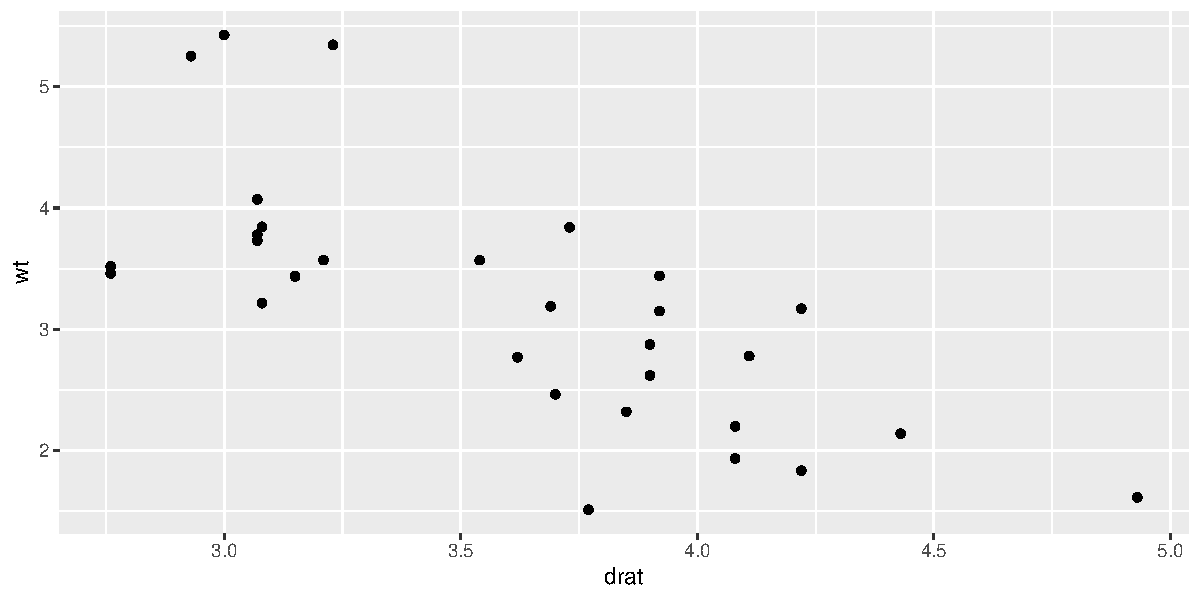
\includegraphics{chapters/01-introduction_files/figure-pdf/fig-1-1.pdf}

}

\caption{\label{fig-1}This is Figure 1, which I made using ggplot2. To
fully appreciate it, I have displayed this image in landscape mode using
the \texttt{\textbackslash{}blandscape} and
\texttt{\textbackslash{}elandscape} commands, from the \texttt{lscape}
LaTeX package`. This feature only works for PDF format.}

\end{figure}%

\elandscape

Integer sed leo ut velit posuere viverra sit amet iaculis augue. Morbi
fermentum arcu augue, ac lobortis metus sagittis et. Nulla faucibus,
mauris non lacinia auctor, odio ex condimentum eros, nec euismod libero
magna vel arcu. In eu purus nunc. Donec tempor, metus eget aliquet
ultricies, felis libero condimentum nulla, hendrerit porta tellus quam
sed purus. Quisque egestas sit amet urna non scelerisque. Quisque
vestibulum sit amet nibh sit amet dignissim. Maecenas semper, elit sit
amet sollicitudin lobortis, urna nisl ullamcorper tortor, et pulvinar
risus ligula a felis. Nullam interdum velit non lectus tempus faucibus.
Aenean vel pellentesque odio. Sed ut leo at purus lobortis fermentum sed
quis ligula. Nullam dictum magna vitae convallis ullamcorper. In ut
varius nunc. Vivamus molestie nibh vel ipsum euismod accumsan. Mauris
bibendum elit quis nisi venenatis, a suscipit leo egestas.

\bookmarksetup{startatroot}

\chapter{The first chapter}\label{the-first-chapter}

Phasellus ultricies rhoncus massa quis dignissim. Praesent pretium,
augue eget iaculis posuere, sem felis cursus orci, at rutrum neque risus
ut sapien. Curabitur in est id neque lacinia fringilla in sit amet
felis. Nunc suscipit est quis neque posuere, laoreet sodales risus
luctus. Vestibulum ultricies interdum dictum. Maecenas sit amet nisi
diam. Aenean enim sapien, vestibulum eget suscipit accumsan, malesuada
id ante. Lorem ipsum dolor sit amet, consectetur adipiscing elit.
Maecenas accumsan magna vel velit egestas feugiat. Fusce sed arcu at
sapien feugiat porttitor in et sem. Phasellus fringilla ornare ipsum.
Maecenas eleifend felis quis fringilla tincidunt. Sed auctor, dui eu
viverra gravida, urna elit semper lorem, in gravida lacus metus ut erat.
Nam vitae imperdiet lacus (see Abbildung~\ref{fig-cudillero}).

\begin{figure}

\centering{

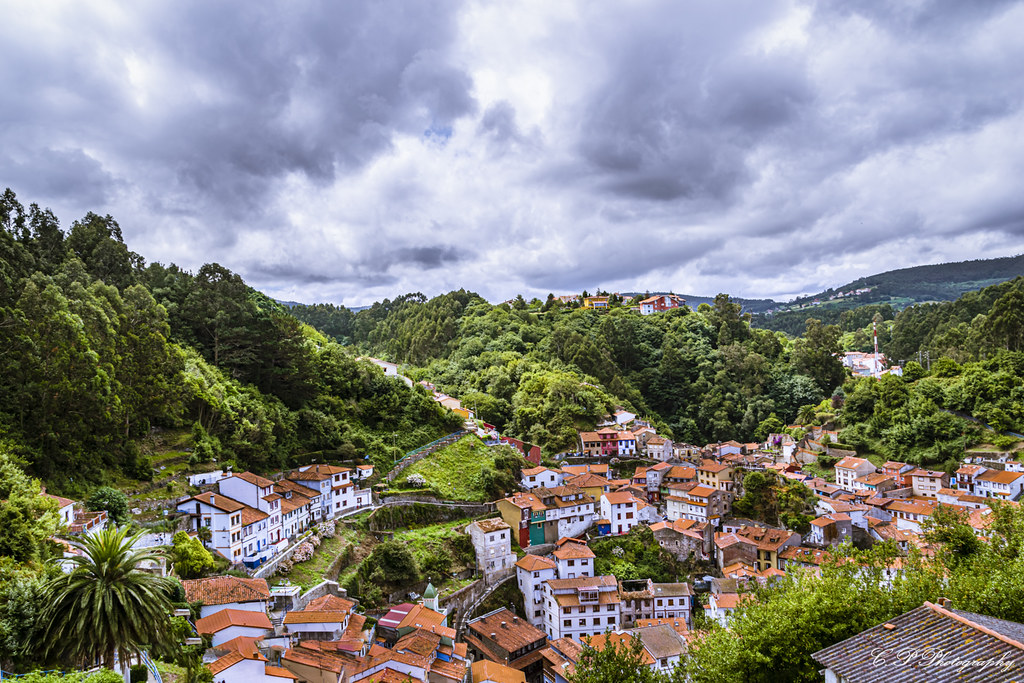
\includegraphics[width=3.64583in,height=3.125in]{chapters/../img/cudillero.jpg}

}

\caption{\label{fig-cudillero}A picture of Cudillero, a village in my
home Asturias (Spain)}

\end{figure}%

\section{Yet another section}\label{yet-another-section}

Ut eu fermentum risus, quis laoreet nisl. Vestibulum feugiat blandit
lectus nec blandit. Mauris interdum sem id nunc interdum facilisis.
Fusce commodo, purus sed gravida pretium, risus mi volutpat enim,
viverra posuere augue enim at velit. Fusce sollicitudin ipsum laoreet
imperdiet tempor. Vestibulum vel dapibus est. Nulla vitae quam congue,
porttitor odio vel, iaculis est. Vestibulum tortor massa, feugiat quis
nunc sed, scelerisque rhoncus dui. Ut non ultrices ligula, vestibulum
faucibus tellus. Sed eu arcu hendrerit, scelerisque mauris vel, commodo
justo.

\begin{Shaded}
\begin{Highlighting}[]
\CommentTok{\# this is some R code}
\NormalTok{a }\OtherTok{\textless{}{-}} \DecValTok{1}
\NormalTok{b }\OtherTok{\textless{}{-}} \DecValTok{2}
\NormalTok{a }\SpecialCharTok{+}\NormalTok{ b}
\end{Highlighting}
\end{Shaded}

\section{Yes, another section}\label{yes-another-section}

Duis eros felis, vestibulum non erat vel, tempor finibus justo. Aliquam
vehicula nisl a dolor interdum aliquet. Fusce maximus dui pellentesque
lorem posuere, id ullamcorper lacus posuere. Sed vel nisl mauris. Donec
eu dignissim urna, id accumsan ipsum. Pellentesque facilisis a justo nec
tempor. Integer sit amet nibh iaculis nisi viverra porta. In viverra
elit eget tincidunt placerat. Cras dolor diam, porta eget purus at,
commodo elementum sem. Aliquam nec semper leo (see
Gleichung~\ref{eq-logistic}).

\begin{equation}\phantomsection\label{eq-logistic}{
f(x)={\frac {L}{1+e^{-k(x-x_{0})}}}
}\end{equation}

\subsection{Finally, a sub-section}\label{finally-a-sub-section}

Donec gravida arcu nec felis viverra placerat. Class aptent taciti
sociosqu ad litora torquent per conubia nostra, per inceptos himenaeos.
Orci varius natoque penatibus et magnis dis parturient montes, nascetur
ridiculus mus. Aliquam ornare ligula sed sagittis ornare. Quisque magna
orci, aliquam vitae nisl non, pellentesque sodales sapien. Donec
eleifend posuere magna, quis convallis orci auctor quis. Vestibulum
vulputate mi vel efficitur egestas.

\begin{quote}
``Suspendisse quis sapien in sem rutrum porttitor sit amet ac lorem.
Mauris gravida augue eu purus faucibus, id accumsan est varius.
Curabitur id ex egestas, sagittis erat id, eleifend nunc.''
\end{quote}

\bookmarksetup{startatroot}

\chapter{The second chapter}\label{the-second-chapter}

Sed eleifend congue aliquam. Aenean risus tellus, tincidunt at venenatis
id, maximus feugiat nunc. Phasellus tellus enim, euismod auctor nisi at,
blandit aliquam ligula. Donec auctor dignissim eros. Etiam et enim diam.
Aenean eget tellus sodales, laoreet risus at, imperdiet mauris. Cras
nulla nulla, vehicula id accumsan vitae, malesuada at neque. Curabitur
suscipit risus at sodales sagittis. Nam molestie sapien tincidunt
placerat semper. Vestibulum ut eleifend urna, at aliquet quam (see
Tabelle~\ref{tbl-1}).

\begin{longtable}{rrrrrrrrrrr}

\toprule
mpg & cyl & disp & hp & drat & wt & qsec & vs & am & gear & carb \\ 
\midrule\addlinespace[2.5pt]
21.0 & 6 & 160 & 110 & 3.90 & 2.620 & 16.46 & 0 & 1 & 4 & 4 \\ 
21.0 & 6 & 160 & 110 & 3.90 & 2.875 & 17.02 & 0 & 1 & 4 & 4 \\ 
22.8 & 4 & 108 & 93 & 3.85 & 2.320 & 18.61 & 1 & 1 & 4 & 1 \\ 
21.4 & 6 & 258 & 110 & 3.08 & 3.215 & 19.44 & 1 & 0 & 3 & 1 \\ 
18.7 & 8 & 360 & 175 & 3.15 & 3.440 & 17.02 & 0 & 0 & 3 & 2 \\ 
18.1 & 6 & 225 & 105 & 2.76 & 3.460 & 20.22 & 1 & 0 & 3 & 1 \\ 
\bottomrule


\caption{\label{tbl-1}This is Table 1, which contains the
\texttt{mtcars} dataset}

\tabularnewline
\end{longtable}

\section{You guessed it, a section}\label{you-guessed-it-a-section}

Integer dui odio, fringilla sit amet consequat a, accumsan ut eros. Sed
mauris risus, laoreet sit amet nunc id, ornare sagittis odio.
Suspendisse elementum laoreet condimentum. Sed molestie mauris diam.
Interdum et malesuada fames ac ante ipsum primis in faucibus. Praesent
blandit at nisl imperdiet sagittis. In at metus sem. Aliquam ultricies
fermentum risus, malesuada auctor nisi elementum quis. Nulla facilisis
aliquet lacus, non aliquam justo volutpat vitae.

Phasellus vitae nisl purus. Nullam sed odio elit. Maecenas gravida
convallis faucibus. Nulla pellentesque, nulla ut efficitur commodo,
tortor nulla aliquet leo, ut commodo enim magna sit amet erat. Lorem
ipsum dolor sit amet, consectetur adipiscing elit. Suspendisse potenti.
Donec euismod eros eu rhoncus mollis. Fusce id enim in sem sodales
tempor eu quis dolor. Nulla sed elit eget ex blandit consequat ac
tincidunt quam\footnote{A footnote!}.Mauris ac sem eget nibh convallis
venenatis. Ut ullamcorper egestas condimentum. Suspendisse ut pharetra
neque. Donec scelerisque at odio et congue. Sed quis turpis at velit
vestibulum sollicitudin eu ut elit. Suspendisse placerat hendrerit
rutrum. Praesent accumsan ligula nec eleifend dapibus.

\bookmarksetup{startatroot}

\chapter{Discussion}\label{discussion}

Aliquam at massa turpis. Donec ac aliquet ligula. Integer eget magna
mauris. Vestibulum venenatis ac risus eu ultrices. Suspendisse fringilla
vestibulum blandit. Integer hendrerit fermentum ante, molestie consequat
risus faucibus nec. Donec pellentesque condimentum bibendum. Cras
suscipit ut elit in ullamcorper. Phasellus egestas arcu quis mi posuere,
vitae commodo lorem mattis. Nulla a risus nec ligula finibus facilisis.
In lorem mauris, pretium at libero et, hendrerit ornare orci. Aliquam
sed odio vel lacus ullamcorper vehicula eget nec purus.

Suspendisse potenti. Sed eget urna ac tortor ornare ullamcorper nec eu
urna. Donec quis auctor metus. Curabitur quis pretium turpis. Sed ut
lobortis nisi. Aenean eu mattis tortor. In ullamcorper interdum lacus eu
euismod. Proin hendrerit lorem ut nibh malesuada, non hendrerit mi
viverra. Aliquam quam nunc, fringilla consectetur imperdiet et,
consectetur id libero. Etiam vestibulum ex vitae neque placerat, nec
eleifend purus euismod. Ut eu magna ipsum. In odio nibh, posuere sit
amet convallis sed, dignissim id ligula. Donec eleifend, massa sit amet
eleifend volutpat, est erat laoreet ligula, dapibus dapibus nulla diam
nec nunc. Orci varius natoque penatibus et magnis dis parturient montes,
nascetur ridiculus mus. Aenean a fringilla dui, eu interdum ex. Mauris
auctor consectetur arcu, id tincidunt odio iaculis sit amet.

\begin{tcolorbox}[enhanced jigsaw, rightrule=.15mm, opacityback=0, bottomtitle=1mm, left=2mm, breakable, colbacktitle=quarto-callout-note-color!10!white, leftrule=.75mm, coltitle=black, title=\textcolor{quarto-callout-note-color}{\faInfo}\hspace{0.5em}{Hinweis}, bottomrule=.15mm, colback=white, toptitle=1mm, toprule=.15mm, colframe=quarto-callout-note-color-frame, titlerule=0mm, arc=.35mm, opacitybacktitle=0.6]

This is a callout note. Check the Quarto documentation on
\href{https://quarto.org/docs/authoring/callouts.html}{callout notes}
for more details.

\end{tcolorbox}

Class aptent taciti sociosqu ad litora torquent per conubia nostra, per
inceptos himenaeos. Fusce efficitur lacus et sem ornare, et elementum
leo imperdiet. Mauris sit amet vehicula lacus. Donec lacinia pharetra
dui et maximus. Ut lobortis sit amet massa consectetur tempus. Duis
mauris erat, semper non eros et, pellentesque aliquam turpis. Etiam
augue libero, iaculis interdum sollicitudin feugiat, sollicitudin vitae
nulla. Aliquam non molestie erat, vel pellentesque eros. Mauris
sagittis, urna id vestibulum bibendum, lectus eros faucibus odio, non
congue ipsum nulla a ante.

Vestibulum vulputate, sapien ut convallis consequat, lorem est
ullamcorper neque, a malesuada arcu sem ac ipsum. Duis ac semper ipsum.
Aliquam eget lorem dignissim, pretium orci non, sollicitudin arcu.
Quisque urna ipsum, tincidunt ac risus eu, suscipit sollicitudin tellus.
Donec eget tortor et neque venenatis vestibulum. In vestibulum massa
vitae arcu maximus consectetur. Phasellus tellus tellus, congue sit amet
nisl vitae, tempus hendrerit nisi. Maecenas ullamcorper quis elit vitae
auctor. Curabitur egestas eleifend justo, et fringilla mauris commodo
ut. Vestibulum maximus neque dolor, at dictum nunc cursus et. Maecenas
ac cursus nulla. Nunc ut massa ex. Suspendisse potenti. Vivamus est
nisi, varius ut arcu eget, iaculis convallis ex. Etiam condimentum magna
mi, et rhoncus nulla efficitur ac. Proin ultricies mattis neque, sed
varius erat.

Donec porttitor facilisis sapien id scelerisque. Aliquam gravida
tristique lobortis. Cras lacinia mattis sapien, a accumsan risus
interdum vitae. Nam diam mauris, sollicitudin eu commodo ut, convallis
sit amet est. Nam volutpat nibh vel orci euismod tempus. Donec in sem
magna. Pellentesque eleifend commodo enim, ut suscipit odio tempus ut.
Nullam tempor turpis sapien, in suscipit quam finibus quis. Class aptent
taciti sociosqu ad litora torquent per conubia nostra, per inceptos
himenaeos. Sed semper orci dolor, finibus ornare odio viverra vel. In
tellus ante, vulputate nec purus ac, feugiat viverra mi.

\clearpage

\bookmarksetup{startatroot}

\chapter*{Bibliography / Inhaltsverzeichnis -\textgreater{} bitte
einfach entsprechend im .qmd
ändern}\label{bibliography-inhaltsverzeichnis---bitte-einfach-entsprechend-im-.qmd-uxe4ndern}
\addcontentsline{toc}{chapter}{Bibliography / Inhaltsverzeichnis
-\textgreater{} bitte einfach entsprechend im .qmd ändern}

\markboth{Bibliography / Inhaltsverzeichnis -\textgreater{} bitte
einfach entsprechend im .qmd ändern}{Bibliography / Inhaltsverzeichnis
-\textgreater{} bitte einfach entsprechend im .qmd ändern}

\phantomsection\label{refs}
\begin{CSLReferences}{1}{0}
\bibitem[\citeproctext]{ref-bolliger2009full}
Bolliger, S. A., Ross, S., Oesterhelweg, L., Thali, M. J., \& Kneubuehl,
B. P. (2009). Are full or empty beer bottles sturdier and does their
fracture-threshold suffice to break the human skull? \emph{Journal of
forensic and legal medicine}, \emph{16}(3), 138--142.

\bibitem[\citeproctext]{ref-wickham2019welcome}
Wickham, H., Averick, M., Bryan, J., Chang, W., McGowan, L. D.,
François, R., Grolemund, G., Hayes, A., Henry, L., Hester, J., et al.
(2019). Welcome to the Tidyverse. \emph{Journal of open source
software}, \emph{4}(43), 1686.

\end{CSLReferences}

\cleardoublepage
\phantomsection
\addcontentsline{toc}{part}{Anhang}
\appendix

\chapter{Einleitung}\label{einleitung-1}

Lorem ipsum dolor sit amet, consectetur adipiscing elit. Integer quis
condimentum lorem. Morbi in metus molestie, gravida lectus eu, rhoncus
arcu. Proin lobortis ullamcorper massa quis volutpat. Pellentesque
sollicitudin, sem vel porta volutpat, ante purus rutrum magna, sed
placerat magna arcu ut metus. Nulla facilisi. Proin quis lorem tempor,
rutrum sapien ut, egestas nisl. Nunc lacus lacus, aliquet sed felis sit
amet, fringilla scelerisque turpis. Fusce semper felis et turpis laoreet
mollis. Duis ullamcorper nisi sem, id sagittis arcu bibendum ac. Quisque
semper nulla a sem placerat suscipit. Aenean vel massa nec erat blandit
accumsan et non felis. Suspendisse nec bibendum ipsum. Fusce eu nibh
convallis, rutrum sapien nec, feugiat ante (Bolliger et al., 2009;
Wickham et al., 2019).

\section{Ein erster Abschnitt}\label{ein-erster-abschnitt-1}

Fusce facilisis est tortor, id iaculis dolor rutrum ac. Curabitur id
bibendum lacus, eget lacinia velit. Fusce suscipit tempus nibh convallis
tempor. Aenean ullamcorper, orci et semper sodales, orci elit rutrum
quam, eget lobortis leo felis in dui. Morbi et odio aliquet ligula
suscipit molestie nec quis libero. Proin tempus gravida neque non
faucibus. Donec hendrerit molestie elit sed congue. Donec faucibus
mollis accumsan. Fusce vestibulum porttitor dui eu facilisis. Aliquam
rutrum erat tortor, eu gravida nisi cursus quis. Nullam dignissim luctus
turpis non ullamcorper. Integer eleifend molestie est, facilisis
suscipit diam. Nullam in justo nisl.

Phasellus vitae tortor eros. Nam eu eros id erat interdum blandit vitae
eu libero. Cras eget dictum eros, id condimentum tellus. Ut sed diam
tristique, aliquam urna eget, auctor tortor. Vestibulum gravida urna in
consectetur volutpat. Maecenas id nisi quis neque dictum ultrices nec
quis tellus. Pellentesque dictum aliquam enim, id efficitur mi vulputate
sit amet. In nec aliquam justo, nec elementum leo.

Sed luctus sit amet diam ac sollicitudin. Suspendisse porttitor augue
elit, ac interdum sapien congue et. Maecenas ut eleifend ex. Phasellus
non felis porttitor, suscipit est non, vulputate eros. Fusce nec mollis
justo. Phasellus non maximus lectus. Integer et lorem mollis, hendrerit
magna at, sagittis purus.

\includegraphics[width=4in,height=0.95in]{appendices/01-test_files/figure-latex/mermaid-figure-1.png}

\section{Ein zweiter Abschnitt}\label{ein-zweiter-abschnitt-1}

Suspendisse maximus mauris in pretium convallis. Cras nec egestas purus.
Suspendisse sodales nisl a nulla varius, vel molestie neque convallis.
Cras aliquam malesuada lectus et rhoncus. Suspendisse aliquam pretium
viverra. Aenean sed lobortis nulla. Ut diam dui, efficitur ac eleifend
ornare, porttitor eget nibh. Quisque euismod quam risus, sit amet
aliquam mauris mollis in.

Curabitur dictum ultrices pulvinar. In id velit vel arcu aliquam
commodo. Quisque eu odio vitae sapien molestie dapibus ut at sapien. In
ac dolor ut neque viverra scelerisque eu in nibh. Quisque ac ex libero.
Praesent posuere sodales enim. Suspendisse lobortis, justo ut vehicula
dapibus, dui libero sodales quam, laoreet mattis mauris urna tempus
diam. Maecenas rhoncus lorem ac finibus interdum. Praesent egestas mi at
tempor pellentesque. Pellentesque faucibus hendrerit odio eget semper.
Proin ultricies libero vitae ligula congue tempor (see
Abbildung~\ref{fig-1}).

\blandscape

\begin{figure}

\centering{

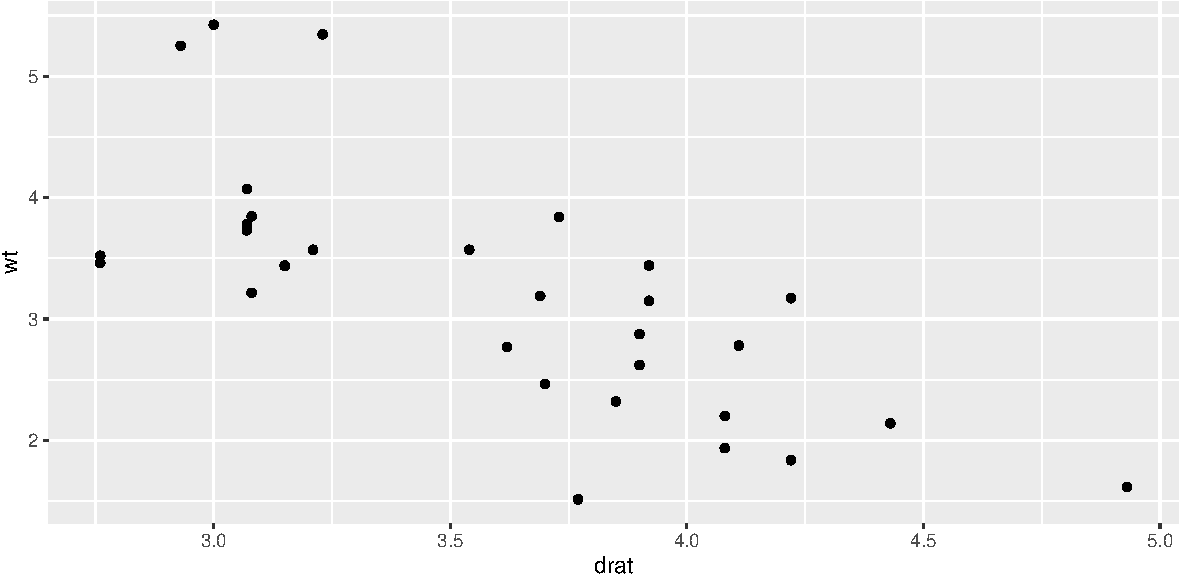
\includegraphics{appendices/01-test_files/figure-pdf/fig-1-1.pdf}

}

\caption{\label{fig-1}This is Figure 1, which I made using ggplot2. To
fully appreciate it, I have displayed this image in landscape mode using
the \texttt{\textbackslash{}blandscape} and
\texttt{\textbackslash{}elandscape} commands, from the \texttt{lscape}
LaTeX package`. This feature only works for PDF format.}

\end{figure}%

\elandscape

Integer sed leo ut velit posuere viverra sit amet iaculis augue. Morbi
fermentum arcu augue, ac lobortis metus sagittis et. Nulla faucibus,
mauris non lacinia auctor, odio ex condimentum eros, nec euismod libero
magna vel arcu. In eu purus nunc. Donec tempor, metus eget aliquet
ultricies, felis libero condimentum nulla, hendrerit porta tellus quam
sed purus. Quisque egestas sit amet urna non scelerisque. Quisque
vestibulum sit amet nibh sit amet dignissim. Maecenas semper, elit sit
amet sollicitudin lobortis, urna nisl ullamcorper tortor, et pulvinar
risus ligula a felis. Nullam interdum velit non lectus tempus faucibus.
Aenean vel pellentesque odio. Sed ut leo at purus lobortis fermentum sed
quis ligula. Nullam dictum magna vitae convallis ullamcorper. In ut
varius nunc. Vivamus molestie nibh vel ipsum euismod accumsan. Mauris
bibendum elit quis nisi venenatis, a suscipit leo egestas.



\end{document}
